\documentclass[a4paper,12pt]{article} 

%%% Работа с русским языком
\usepackage{cmap}					% поиск в PDF
\usepackage{mathtext} 				% русские буквы в фомулах
\usepackage[T2A]{fontenc}			% кодировка
\usepackage[utf8]{inputenc}			% кодировка исходного текста
\usepackage[english,russian]{babel}	% локализация и переносы

%%% Дополнительная работа с математикой
\usepackage{amsmath,amsfonts,amssymb,amsthm,mathtools, gensymb} % AMS
\usepackage{icomma} % "Умная" запятая: $0,2$    ф--- число, $0, 2$ --- перечисление

%%Таблица
\usepackage[table,xcdraw]{xcolor}
\usepackage{caption}
\usepackage{floatrow}
\floatsetup[table]{capposition=top}
\floatsetup[wrapfigure]{capposition=bottom}
\usepackage{multirow}

\usepackage{hyperref}

%Отступы и поля 
\textwidth=18cm
\oddsidemargin=-1cm
\topmargin=-2cm
\textheight=25cm


%% Номера формул
\mathtoolsset{showonlyrefs=false} % Показывать номера только у тех формул, на которые есть \ref{} в тексте.

%% Шрифты
\usepackage{euscript}	 % Шрифт Евклид
\usepackage{mathrsfs} % Красивый матшрифт

%% Свои команды
\DeclareMathOperator{\sgn}{\mathop{sgn}}

%% Перенос знаков в формулах (по Львовскому)
\newcommand*{\hm}[1]{#1\nobreak\discretionary{}
{\hbox{$\mathsurround=0pt #1$}}{}}

%% Стиль страницы
\usepackage{fancyhdr}

%% Для рисунков
\usepackage{graphicx}
\usepackage[export]{adjustbox}
\usepackage{float}
\usepackage{ragged2e}
\usepackage{wrapfig}

\pagestyle{fancy}
\begin{document}
\begin{titlepage}
\begin{center}
%\vspace*{1cm}
\large{\small ФЕДЕРАЛЬНОЕ ГОСУДАРСТВЕННОЕ АВТОНОМНОЕ ОБРАЗОВАТЕЛЬНОЕ\\ УЧРЕЖДЕНИЕ ВЫСШЕГО ОБРАЗОВАНИЯ \\ МОСКОВСКИЙ ФИЗИКО-ТЕХНИЧЕСКИЙ ИНСТИТУТ\\ (НАЦИОНАЛЬНЫЙ ИССЛЕДОВАТЕЛЬСКИЙ УНИВЕРСИТЕТ)\\ ФАКУЛЬТЕТ АЭРОКОСМИЧЕСКИХ ТЕХНОЛОГИЙ}
\vfill
\line(1,0){490}\\[1mm]
\huge{Лабораторная работа 1.2}\\
\huge\textbf{Исследование эффекта Комптона}\\
\line(1,0){490}\\[1mm]
\vfill
\begin{flushright}
\normalsize{Рогозин Владимир}\\
\normalsize{\textbf{Группа Б03-106}}\\
\end{flushright}
\end{center}
\end{titlepage}
\fancyhead[L] {Работа 1.2}

\textbf{Цель работы}:
с помощью сцинтилляционного спектрометра исследовать энергетический спектр $\gamma$-квантов, рассеянных на графите. Определить энергию рассеянных $\gamma$-квантов в зависимости от угла рассеяния, а также энергию покоя частиц, на которых происходит комптоновское рассеяние.


% \textbf{Оборудование}:
% лазер; кассета с набором сеток разного
% периода; линзы; щель с микрометрическим винтом; оптический стол
% c набором рейтеров и крепёжных винтов; экран; линейка.


\section{Теоретические сведения}
Рассеяние $\gamma$-лучей в веществе относится к числу явлений, в которых особенно ясно проявляется двойственная природа излучения. Волновая теория, хорошо объясняющая рассеяние длинноволнового излучения, испытывает трудности при описании рассеяния рентгеновских и $\gamma$-лучей. Эта теория, в частности, не может объяснить, почему в составе рассеянного излучения, измеренного Комптоном, кроме исходной волны с частотой $\omega_0$ появляется дополнительная длинноволновая компонента, отсутствующая в спектре первичного излучения.

Появление этой компоненты легко объяснимо, если считать, что $\gamma$-излучение представляет собой поток квантов (фотонов), имеющих энергию $\hbar\omega$ и импульс $p = \hbar\omega / c$. Эффект Комптона -- увеличение длины волны рассеянного излучения по сравнению с падающим -- интерпретируется как результат упругого соударения двух частиц: $\gamma$-кванта (фотона) и свободного электрона.

Рассмотрим элементарную теорию эффекта Комптона. Пусть электрон до соударения покоился,
а $\gamma$-квант имел начальную энергию $\hbar\omega_0$ и импульс $\hbar\omega_0 / c$. После соударения электрон приобретает энергию $\gamma mc^2$ и импульс $\gamma mv$, где $\gamma = (1 - \beta^2)^{-1 / 2}$, $\beta = v/c$, а $\gamma$-квант рассеивается на некоторый угол $\theta$ по отношению к первоначальному направлению движения. Энергия и импульс $\gamma$-кванта становятся соответственно равными $\hbar\omega_1$ и $\hbar\omega_1 / c$.

Запишем для рассматриваемого процесса законы сохранения энергии
и импульса:
\begin{equation}\label{eq: Energy conservation law}
    mc^2 + \hbar\omega_0 = \gamma mc^2 + \hbar\omega_1, 
\end{equation}
\begin{equation}\label{eq: Impulse oX conservation law}
    \hbar\omega_0 / c = \gamma mv\cos\varphi + \hbar\omega_1 / c \cos\theta, 
\end{equation}
\begin{equation}\label{eq: Impulse oY conservation law}
    \gamma mv\sin\varphi = \hbar\omega_1 / c \sin\theta. 
\end{equation}

Решая совместно эти уравнения, нетрудно получить, что изменение длины волны
рассеянного излучения равно
\begin{equation}\label{eq: Wave length difference}
    \Delta\lambda = \lambda_1 - \lambda_0 = \frac{h}{mc}(1 - \cos\theta) = \Lambda_K(1 - \cos\theta),
\end{equation}

\begin{wrapfigure}[12]{r}{0.5\textwidth}\label{fig: Collision model}
    \begin{center}
    \vspace{-20pt}
        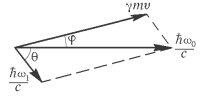
\includegraphics[width = 0.8\textwidth]{Collision model.png}
    \end{center}
    \caption{Векторная диаграмма рассеяния $\gamma$-кванта на электроне}
\end{wrapfigure}
где $\lambda_0$ и $\lambda_1$ -- длины волн $\gamma$-кванта до и после рассеяния, а величина $\Lambda_K$ называется комптоновской длиной волны электрона.  Из формулы (\ref{eq: Wave length difference}) следует, что комптоновское смещение не зависит ни от длины волны первичного излучения, ни от рода вещества, в котором наблюдается рассеяние. В приведенном выводе электрон в атоме считается свободным. Для $\gamma$-квантов с энергией в несколько десятков, а тем более сотен килоэлектрон-вольт, связь электронов в атоме, действительно, мало существенна, так как энергия их связи в легких атомах не превосходит нескольких килоэлектрон-вольт, а для большинства электронов еще меньше.

При рассеянии на связанных электронах изменение импульса кванта воспринимается атомом в целом. Поскольку масса атома очень велика, передача импульса не сопровождается сколь-нибудь заметной передачей энергии, и наблюдается несмещенная (по энергии) компонента в спектре рассеянного излучения. Таким образом, рассеяние
$\gamma$-квантов на связанных электронах можно рассматривать как упругое столкновение квантов с атомами. В классике такое рассеяние называется рэлеевским и рассматривается как процесс, при котором связанные
электроны атома приходят в резонансное колебание под действием падающего излучения, а затем сами излучают фотоны той же частоты. При рассеянии квантов не очень высокой энергии (1 ÷ 10 кэВ) часть электронов ведет себя, как свободные, а часть -- как связанные. Оба типа рассеяния при этом наблюдаются одновременно.

При увеличении атомного номера $Z$ рассеивателя сечение рэлеевского рассеяния растет как $Z^2$, тогда как сечение комптоновского рассеяния на атоме пропорционально $Z$. Это происходит по следующей причине. При комптоновском рассеянии каждый электрон атома ведет себя независимо от других, поскольку рассеяние в
этом случае происходит на каком-либо одном из атомных электронов. При рэлеевском рассеянии фотоны излучаются всеми (или почти всеми) электронами атомной оболочки, колеблющимися синфазно. Их излучение когерентно, так что складываются амплитуды, а не интенсивности излученных волн электронов. Сечения комптоновского и рэлеевского рассеяний по-разному зависят и от энергии фотонов. С увеличением энергии сечение рэлеевского рассеяния уменьшается очень быстро, а сечение комптоновского рассеяния -- незначительно.

Кроме рассеяния $\gamma$-кванты испытывают в среде поглощение, вызываемое фотоэффектом и рождением электронпозитронных пар. Процесс рождения пар пороговый, он возможен лишь при энергии $\gamma$-квантов больше $2mc^2 = 1,02$ МэВ и в рассматриваемом энергетическом диапазоне не происходит. При фотоэффекте из атома выбивается электрон, а квант поглощается. Импульс кванта делится между вылетевшим электроном и атомом, а его энергия частично передается электрону, а частично тратится на возбуждение атома. Атом
практически мгновенно (за время порядка $10^{-8}$ с) возвращается в нормальное состояние. Его энергия возбуждения либо излучается в виде мягкого фотона, либо передается какому-нибудь другому электрону, который покидает атом. И в том, и в другом случае энергия возбуждения обычно поглощается соседними атомами рассеивателя.

Основной целью данной работы является проверка соотношения (\ref{eq: Wave length difference}). После перехода от длин волн к энергиям $\gamma$-квантов, соотношение принимает вид
\begin{equation}\label{eq: Energy difference}
    \frac{1}{\varepsilon(\theta)} - \frac{1}{\varepsilon_0} = 1 - \cos\theta.
\end{equation}

Здесь $\varepsilon_0 = E_0 / (mc^2)$ -- выраженная в единицах $mc^2$ энергия $\gamma$-квантов, падающих на рассеиватель, $\varepsilon(\theta)$ -- выраженная в тех же единицах энергия квантов, испытавших комптоновское рассеяние на угол $\theta$, $m$ -- масса электрона.


\section{Экспериментальная установка}
Блок-схема установки изображена на рис. \hyperref[fig: Experimental setup]{2}. Источником излучения \textit{1} служит $^{137}$Cs, испускающий $\gamma$-лучи с энергией $662$ кэВ. Он помещен в толстостенный свинцовый контейнер с коллиматором. Сформированный коллиматором узкий пучок $\gamma$-квантов попадает на графитовую мишень \textit{2} (цилиндр диаметром $40$ мм и высотой $100$ мм).
\begin{figure}[H]\label{fig: Experimental setup}
    \centering
    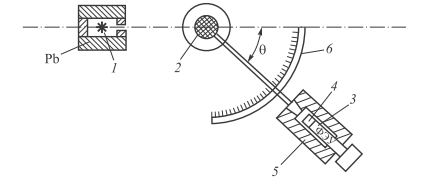
\includegraphics[width = 0.9\textwidth]{Experimental setup.png}
    \caption{Блок-схема установки по изучению рассеяния $\gamma$-квантов}
\end{figure}\

Кванты, испытавшие комптоновское рассеяние в мишени, регистрируются сцинтилляционным счетчиком. Счетчик состоит из фотоэлектронного умножителя \textit{3} (ФЭУ) и сцинтиллятора \textit{4}. Сцинтиллятором служит кристалл NaI(Tl) цилиндрической формы диаметром $40$ мм и высотой $40$ мм, его выходное окно находится в оптическом контакте с фотокатодом ФЭУ. Сигналы, возникающие на аноде ФЭУ, подаются на ЭВМ для
амплитудного анализа. Кристалл и ФЭУ расположены в светонепроницаемом блоке, укрепленном на горизонтальной штанге. Штанга вместе с этим блоком может вращаться относительно мишени, угол поворота отсчитывается по лимбу \textit{6}.

Головная часть сцинтилляционного блока закрыта свинцовым коллиматором \textit{5}, который формирует входной пучок и защищает детектор от постороннего излучения. Основной вклад в это излучение вносят $\gamma$-кванты, проходящие из источника \textit{1} через 6-сантиметровые стенки защитного контейнера. Этот фон особенно заметен при исследовании
комптоновского рассеяния на большие углы ($\approx 120\degree$), когда расстояние между детектором и источником уменьшается.

На рис. \hyperref[fig: Measuring complex]{3} представлена функциональная блок-схема измерительного комплекса, который состоит из ФЭУ, питаемого от высоковольтного выпрямителя ВСВ, обеспечивающего работу ФЭУ в спектрометрическом режиме, усилителя-анализатора УА, являющегося входным интерфейсом ЭВМ, управляемой с клавиатуры КЛ. В ходе проведения эксперимента информация отражается на экране дисплея Д, окончательные результаты в виде таблиц и графиков могут быть выведены на принтер ПР.

\begin{wrapfigure}[12]{l}{0.45\textwidth}\label{fig: Measuring complex}
    \begin{center}
    \vspace{-20pt}
        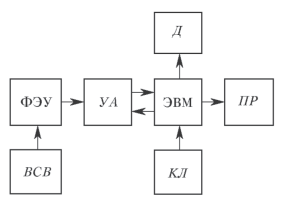
\includegraphics[width = 0.78\textwidth]{Measuring complex.png}
    \end{center}
    \caption{Блок-схема измерительного комплекса}
\end{wrapfigure}
При работе ФЭУ в спектрометрическом режиме величина выходного электрического импульса, снимаемого с анода ФЭУ, пропорциональна энергии регистрируемого $\gamma$-кванта. Световая вспышка в сцинтилляторе вызывается не самими $\gamma$-квантами, а образующимися в кристалле под действием $\gamma$-квантов электронами. Процесс преобразования энергии $\gamma$-кванта в определенное число фотонов на выходе сцинтиллятора состоит из трех стадий: рождение быстрых электронов, возбуждение атомов и молекул сцинтиллятора этими электронами и излучение световых фотонов возбужденными атомами и молекулами. Существуют три механизма взаимодействия $\gamma$-квантов с веществом: комптоновское рассеяние, фотоэффект и рождение электрон-позитронных пар (в нашем случае этот механизм не реализуется, так как энергия $\gamma$-квантов не превосходит порог рождения пар $1,02$ МэВ). Во всех этих случаях в веществе появляется быстрый электрон, который за счет кулоновского взаимодействия эффективно возбуждает на своем пути атомы и молекулы. Число возбужденных центров пропорционально энергии электрона.

Только при фотоэффекте $\gamma$-квант целиком поглощается атомом, а один из электронов внутренней оболочки -- чаще всего K-оболочки -- выбрасывается за пределы атома, унося всю переданную $\gamma$-квантом энергию и теряя ее затем в кристалле. В результате амплитуда световых вспышек оказывается пропорциональной полной энергии первичных $\gamma$-квантов. Комптоновское рассеяние $\gamma$-квантов в кристалле происходит на слабосвязанных электронах. При этом электрону передается только часть энергии $\gamma$-кванта, а оставшаяся часть уносится рассеянным $\gamma$-квантом.

\begin{wrapfigure}[16]{r}{0.5\textwidth}\label{fig: Histogramm example}
    \begin{center}
    \vspace{-20pt}
        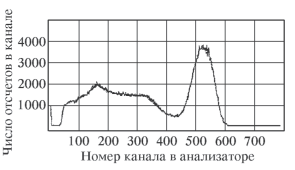
\includegraphics[width = 0.9\textwidth]{Histogramm example.png}
    \end{center}
    \caption{Амплитудное распределение импульсов, возникающих под действием монохроматических $\gamma$-квантов в сцинтилляторе NaI(Tl)}
\end{wrapfigure}
Таким образом, под действием монохроматического излучения на выходе ФЭУ возникает распределение электрических импульсов, показанное на рис. \hyperref[fig: Histogramm example]{4}. В амплитудном распределении импульсов имеется так называемый фотопик, возникающий в результате фотоэффекта, и обязанное комптоновскому рассеянию сплошное распределение. Нас будет интересовать положение (номер канала) вершины этого пика в зависимости от угла поворота детектора. Ширина фотопика является аппаратурной, а не истинной, и зависит от характеристик конкретного кристалла и фотоумножителя, используемых в данной работе. Для определения энергии $\gamma$-квантов нужно исследовать кривую распределения
энергетических потерь в кристалле, т. е. распределение по амплитуде
электрических импульсов на выходе ФЭУ. Такое распределение измеряется в данной работе с помощью компьютера, работающего в режиме амплитудного анализатора.

При регистрации $\gamma$-квантов под углом $0\degree$ в спектре излучения присутствуют только $\gamma$-кванты первичной энергии ($662$ кэВ). При увеличении угла регистрируется рассеянное излучение, сдвинутое в соответствии с формулой (\ref{eq: Wave length difference}) в область меньших энергий. Следует подчеркнуть, что при достаточно большой энергии $\gamma$-квантов ($E_\gamma \geq mc^2$), как это имеет место в нашем случае, вероятность рэлеевского рассеяния очень мала и в наблюдаемом спектре рассеяния отсутствует несмещенная линия. При дальнейшем увеличении угла фотопик все дальше отходит от положения фотопика, соответствующего первичному излучению, и все сильнее размывается.

Слева от фотопика после большого провала начинается непрерывный
спектр комптоновских электронов. Этот фон сохраняется при любом
угле рассеяния и мешает определению фотопика рассеянных $\gamma$-квантов.

Регистрация поступающих после ФЭУ импульсов происходит следующим образом. Усилитель-анализатор УА каждому приходящему на его вход импульсу ставит в соответствие с его амплитудой число $i$ от $0$ до $1023$, а затем ЭВМ прибавляет единицу в $i$-ю ячейку памяти. Таким образом, в памяти компьютера происходит накопление числа пришедших
импульсов в соответствии с их амплитудой. На каждое преобразование затрачивается около $20$ мкс, в течение этого времени система «не чувствует» приходящие от ФЭУ импульсы -- это мертвое время счетной аппаратуры. Таким образом, за одну секунду может быть зафиксировано не более $50$ тысяч импульсов. При помощи специальной программы содержание всех $1024$ ячеек памяти периодически выводится на экран дисплея в виде гистограммы, по оси абсцисс которой откладывается амплитуда анализируемого импульса, а по оси ординат -- число импульсов заданной амплитуды. Точность определения положения фотопика составляет примерно $1\%$.


\section{Обработка данных}

\subsection{Проверка функционирования установки}
\begin{enumerate}
    \item
    Включим измерительные устройства и компьютер, запустим программу и войдём в режим измерения спектра. Проверим функционирование установки в этом режиме: при увеличении угла отклонения фотопик должен смещаться влево, в сторону меньших энергий.
    \item 
    Подберём напряжение так, чтобы при нулевом угле $\theta =0\degree$ фотопик был смещен на экране максимально вправо. Дальнейшие измерения были проведены при напряжении $V = 1,2$ В.
\end{enumerate}

\subsection{Измерение зависимости положения фотопика от угла рассеяния}
\begin{enumerate}
    \item
    Снимем зависимость номера канала фотопика от значения угла $\theta$ отклонения счётчика от положения $\theta = 0\degree$, погрешность определения угла составляет $\sigma_\theta = 1\degree$. Систематическая погрешность определения номера канала $N$ составляет $1\%$. Результаты измерений приведены в таблице ниже. 
    \begin{table}[H]\label{tab: data}
        \centering
        \begin{tabular}{|
            >{\columncolor[HTML]{FFFFFF}}c |
            >{\columncolor[HTML]{FFFFFF}}c |
            >{\columncolor[HTML]{FFFFFF}}c |}
            \hline
            {\color[HTML]{000000} $\theta$, $\degree$} & {\color[HTML]{000000} Номер канала фотопика} & {\color[HTML]{000000} Погрешность номера канала} \\ \hline
            {\color[HTML]{000000} 0}   & {\color[HTML]{000000} 920} & {\color[HTML]{000000} --}         \\ \hline
            {\color[HTML]{000000} 10}  & {\color[HTML]{000000} 912} & {\color[HTML]{000000} --}         \\ \hline
            {\color[HTML]{000000} 20}  & {\color[HTML]{000000} 812} & {\color[HTML]{000000} 790 -- 840} \\ \hline
            {\color[HTML]{000000} 30}  & {\color[HTML]{000000} 760} & {\color[HTML]{000000} 740 -- 790} \\ \hline
            {\color[HTML]{000000} 40}  & {\color[HTML]{000000} 691} & {\color[HTML]{000000} 648 -- 735} \\ \hline
            {\color[HTML]{000000} 50}  & {\color[HTML]{000000} 583} & {\color[HTML]{000000} 545 -- 615} \\ \hline
            {\color[HTML]{000000} 60}  & {\color[HTML]{000000} 533} & {\color[HTML]{000000} 500 -- 570} \\ \hline
            {\color[HTML]{000000} 70}  & {\color[HTML]{000000} 478} & {\color[HTML]{000000} 450 -- 505} \\ \hline
            {\color[HTML]{000000} 80}  & {\color[HTML]{000000} 425} & {\color[HTML]{000000} --}         \\ \hline
            {\color[HTML]{000000} 90}  & {\color[HTML]{000000} 389} & {\color[HTML]{000000} --}         \\ \hline
            {\color[HTML]{000000} 100} & {\color[HTML]{000000} 357} & {\color[HTML]{000000} --}         \\ \hline
            {\color[HTML]{000000} 110} & {\color[HTML]{000000} 329} & {\color[HTML]{000000} --}         \\ \hline
            {\color[HTML]{000000} 120} & {\color[HTML]{000000} 304} & {\color[HTML]{000000} --}         \\ \hline
        \end{tabular}
        \caption{Данные положения фотопика при различных углах}
    \end{table}
    \item 
    По данным из таблице построим график зависимости $1 / N$ от ($1 - \cos\theta$), где $N$ -- номер канала фотопика.
\end{enumerate}

\subsection{Определение энергии покоя рассеивающей частицы}
\begin{enumerate}
    \item 
    Двумя способами, определим энергию покоя частицы (электрона), на которой происходит комптоновское рассеяние первичных $\gamma$-квантов. Для этого перепишем соотношение (\ref{eq: Energy difference})в виде:
    \begin{equation}\label{eq: Canal number difference}
        \frac{1}{N(\theta)} - \frac{1}{N(0)} = A \cdot (1 - \cos\theta),
    \end{equation}
    где $A$ -- коэффициент пропорциональности между $\varepsilon(\theta)$ и $N(\theta)$. Энергия покоя частицы найдётся с помощью
    \begin{equation}\label{eq: Electron energy}
        mc^2 = E(0)\frac{E(90)}{E(0) - E(90)} = E_\gamma\frac{N(90)}{N(0) - N(90)},
    \end{equation}
    здесь $E_\gamma = E(0)$ -- энергия электронов, рассеянных вперед, -- просто равна энергии $\gamma$-лучей, испускаемых источником и равна $E_\gamma = 662$ кэВ. Результаты расчётов представлены ниже.

    Погрешность рассчитывалась по формуле 
    \[\sigma_{E_0}^2 = \frac{E_\gamma^2}{(N_0 - N_{90})^4} \cdot (N_{90}^2 \sigma_{N_0}^2 + N_0^2 \sigma_{N_{90}}^2),\]
    где $N_0 = N(0)$ и $N_{90} = N(90)$.
    \begin{table}[H]\label{tab: mc2 result}
        \centering
        \begin{tabular}{|
            >{\columncolor[HTML]{FFFFFF}}c |
            >{\columncolor[HTML]{FFFFFF}}c |
            >{\columncolor[HTML]{FFFFFF}}c |
            >{\columncolor[HTML]{FFFFFF}}c |}
            \hline
            {\color[HTML]{000000} } &
              {\color[HTML]{000000} Результат по измерениям} &
              {\color[HTML]{000000} Результат по аппроксимации} &
              {\color[HTML]{000000} Истинное значение} \\ \hline
            {\color[HTML]{000000} $E_0 = mc^2$, кэВ} &
              {\color[HTML]{000000} $485,0 \pm 11,9$} &
              {\color[HTML]{000000} $515,2$} &
              {\color[HTML]{000000} $511$} \\ \hline
            {\color[HTML]{000000} $\varepsilon_{E_0}$, \%} &
              {\color[HTML]{000000} $2,45$} &
              {\color[HTML]{000000} --} &
              {\color[HTML]{000000} --} \\ \hline
        \end{tabular}
        \caption{Результаты вычислений массы покоя}
    \end{table}
\end{enumerate}


\section{Вывод}
В данной работе исследовалось явление рассеяния фотонов на свободных электронах. В результате удалось:
\begin{itemize}
    \item
    снять зависимость энергии рассеяных фотонов от угла наблюдения. По этим данным, с помощью построенного графика, удалось проверить кооректность основной в данной работе формулы (\ref{eq: Energy difference}). Точки с хорошей точностью легли на прямую.
    
    \item
    двумя способами определить энергию покоя электрона: с помощью значений, полученных экспериментально, и значений, полученных из аппроксимации экспериментальных данных. В первом случае отклонение от табличного значения получилось порядка $7\%$, во втором случае отклонение составило менее $1\%$.
    
\end{itemize}

\newpage
%%%%%%%%%%%%%%%%%%%%%%%%% Графики

\begin{figure}[H]\label{fig: 1divN(1 - cosTheta)}
    \centering
    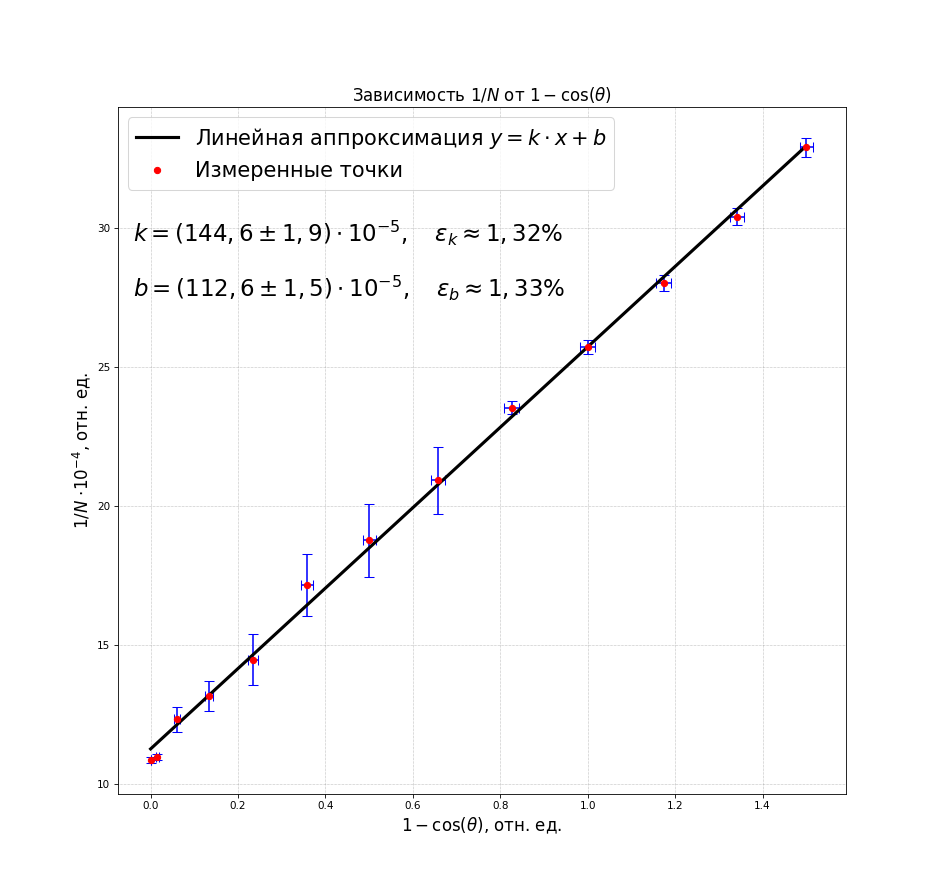
\includegraphics[width = \textwidth]{1divN(1 - cosTheta).png}
\end{figure}
\[k = (144,6 \pm 1,9)\cdot 10^{-5}, \quad \varepsilon_k \approx 1,32\%, \]
\[b = (112,6 \pm 1,5)\cdot 10^{-5}, \quad \varepsilon_b \approx 1,33\%. \]

Погрешности величины по осям $X$, $Y$ вычислялась с использованием соотношения 
\[u = f(x) \Rightarrow \sigma_u = \bigg|\frac{\partial f}{\partial x}\bigg| \sigma_x. \]

Погрешность величины по оси $Y$ состоит из систематической и случайной частей и вычисляется по формуле
\[\sigma_y^2 = \sigma_{\text{сист.}}^2 + \sigma_{\text{случ.}}^2. \]
Систематическая погрешность определения номера канала $N$ составляет $1\%$.

%%%%%%%%%%%%%%%%%%%%%%%%%
\end{document}
